
\section{User study \& Methods}
\textcolor{green}{With this study, we wanted to find out whether the experience of agency can be preserved during physical action augmentation when the user's own brain signals serve as the control signal to a physical end effector. Therefore, we conducted a user study comparing three conditions of agency experience. With the first two conditions, INTENTION and EXTERNAL we queried users at the two edges of agency experience. In EXTERNAL participants had no intention to move and no control over their movement. On the other hand, in INTENTION, participants were acting as they would in their day-to-day lives, fully in control. We then investigated in a third condition where our AUGMENTED prototype sits on the spectrum between INTENTION and EXTERNAL, in other words, whether it preserved agency and to what degree. To answer our question, we employed a mixed methods approach including a psychometric test of intentional binding, one standardized question, and a qualitative (phenomenological) interview.}

\textcolor{red}{With this study, we wanted to find out whether the experience of agency can be preserved during physical action augmentation when the user’s own brain signals serve as the control signal to a physical end effector. To this end, we assessed whether our prototype preserved agency using a mixed methods approach including a psychometric test of intentional binding, one standardized question, and a qualitative (phenomenological) interview.}

\subsection{Participants}
Nine participants (M = 30.00 years, SD = 3.81) were recruited from our local institution and through the institute's online participant pool. All participants were right-handed. Participants were compensated with course credit or 12 Euro per hour of study participation. Prior to their participation, they were informed of the nature of the experiment, recording, and anonymization procedures and signed a consent form. The experiment was approved by the ethics committee of [anonymized]. One participant had to be excluded from further data analyses due to significant deviations from the instructions in the execution of the task.
%the Department of Psychology and Ergonomics at TU Berlin (tracking number: BPN\_GEH\_2\_230130220421).

% \begin{figure*}
%     \centering
%     \includegraphics[width=\textwidth]{figures/task_design.png}
%     \caption{(a) description of the experimental conditions, (b) their hypothesized effects on sense of agency from the perspective of a comparator model, is inspired by~\citet{Dewey2019-dg} (c) depicts the flow of movement generation in the participant and the system between conditions.}
%     \label{fig:task_design}
% \end{figure*}

\subsection{Apparatus}
The experimental setup, depicted in Figure~\ref{fig:setup}, comprised: (1) a 1-channel EMG device, (2) a 64-channel EEG system, (3) a medically-compliant EMS device connected to two electrodes worn on the forearm, and (4) a tablet to run the experiment and collect behavioral responses. To assist readers in replicating our experiment, we provide the necessary technical details, the complete source code for the experiment, the collected data, and the analysis scripts\footnote{[anonymized]}.
% TODO add links after anonymization is lifted.

\begin{figure}[!h]
    \centering
    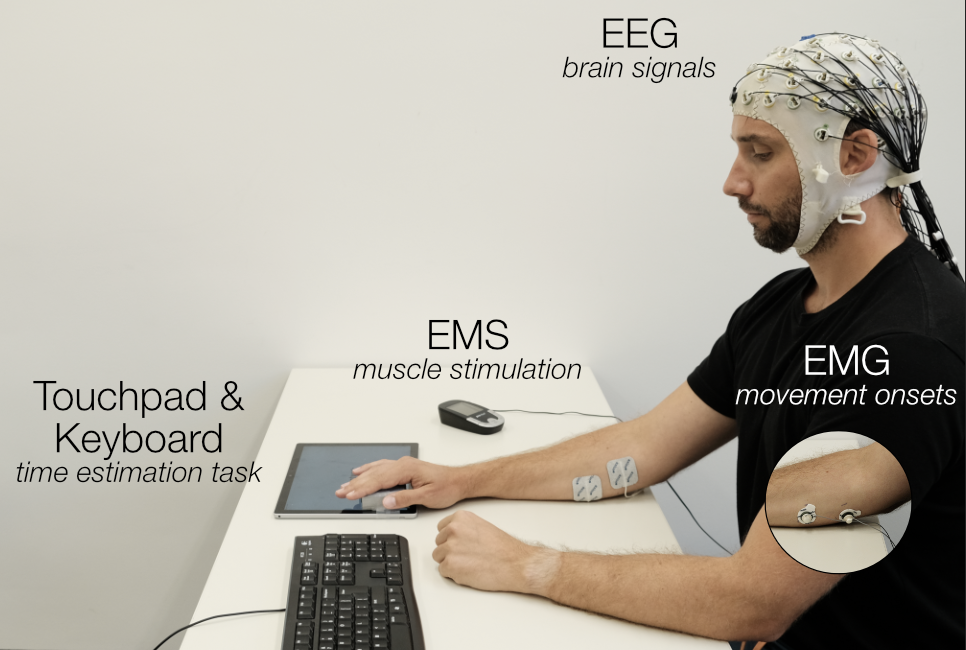
\includegraphics[width=\columnwidth]{figures/setup_fixed.png}
    \caption{Experimental setup of measurement-- and input devices (image with consent from participant).}
    \label{fig:setup}
\end{figure}

\indent\textbf{(1) EMG Recording.} EMG data was recorded from 1 bipolar channel using the BrainAmp ExG amplifier (BrainProducts GmbH, Gilching, Germany). The two electrodes were placed above the flexor digitorum profundus with a reference electrode located on the wrist bone. EMG data was collected in synchrony with the EEG data through BrainProducts' BrainVision Recorder. \textcolor{green}{EMG data was only recorded for the first experimental condition to obtain labels for classifier training. After that, the EMG electrodes were changed for EMS electrodes.}

\indent\textbf{(2) EEG Recording.} EEG data was recorded from 64 actively amplified Ag/AgCl electrodes referenced to \textcolor{green}{electrode FCz} in an actiCap Snap cap using BrainAmp DC amplifiers from BrainProducts. Electrodes were placed according to the extended international 10–20 system \cite{Jasper1983-uw}. One electrode was placed under the right eye to provide additional information about eye movements (vEOG). After fitting the cap, all electrodes were filled with conductive gel to ensure proper conductivity, and electrode impedance was brought below 10k$\Omega$. EEG (and EMG) data were recorded with a sampling rate of 250 Hz. 

We used LSL\footnote{https://github.com/sccn/labstreaminglayer} to make the data streams available in the network and synchronize the recordings of EEG/EMG data and an experiment marker stream that marked sections of the study procedure.

\indent\textbf{(3) Electrical Muscle Stimulation.} We actuated the ring finger via EMS, which was delivered with two electrodes attached to the participants' flexor digitorum profundus muscle. We utilized the flexor digitorum profundus since we found that we can robustly actuate it without inducing unintended motion of neighboring fingers. This finger actuation was achieved via a medically compliant battery-powered muscle stimulator (TENS/EMS Super Duo Plus, prorelax, Düren, Germany). The EMS system's output was controlled by flipping a solid state relay (silent) connected via an Arduino Uno (Arduino, Monza, Italy) to the experiment computer. The EMS was pre-calibrated by the participant to ensure a pain-free but effective stimulation and robust actuation leading to an `immediate' tap on the touchscreen after actuation. To ensure a comfortable experimental experience so that participants relaxed their arm musculature as much as possible, a custom built hand rest (support device) was placed on top of the touchscreen for participants, see figure~\ref{fig:setup}.

\indent\textbf{(4) Experiment Presentation and Collection of Behavioral Responses.} An Acer Group (Acer Inc, Taipeh, Taiwan) tablet was used to present the task to participants and record their behavioral responses. In addition to the tablet, we used an external keyboard to allow \textcolor{red}{response input of users indicating}~\textcolor{green}{users to input} their timing judgements.

\subsection{Experimental Task, Design and Procedure}
Participants performed a simple tapping task in three conditions with 75 trials each: INTENTION, EXTERNAL, and AUGMENTED, see figure~\ref{fig:task_design}.

\begin{figure}
    \centering
    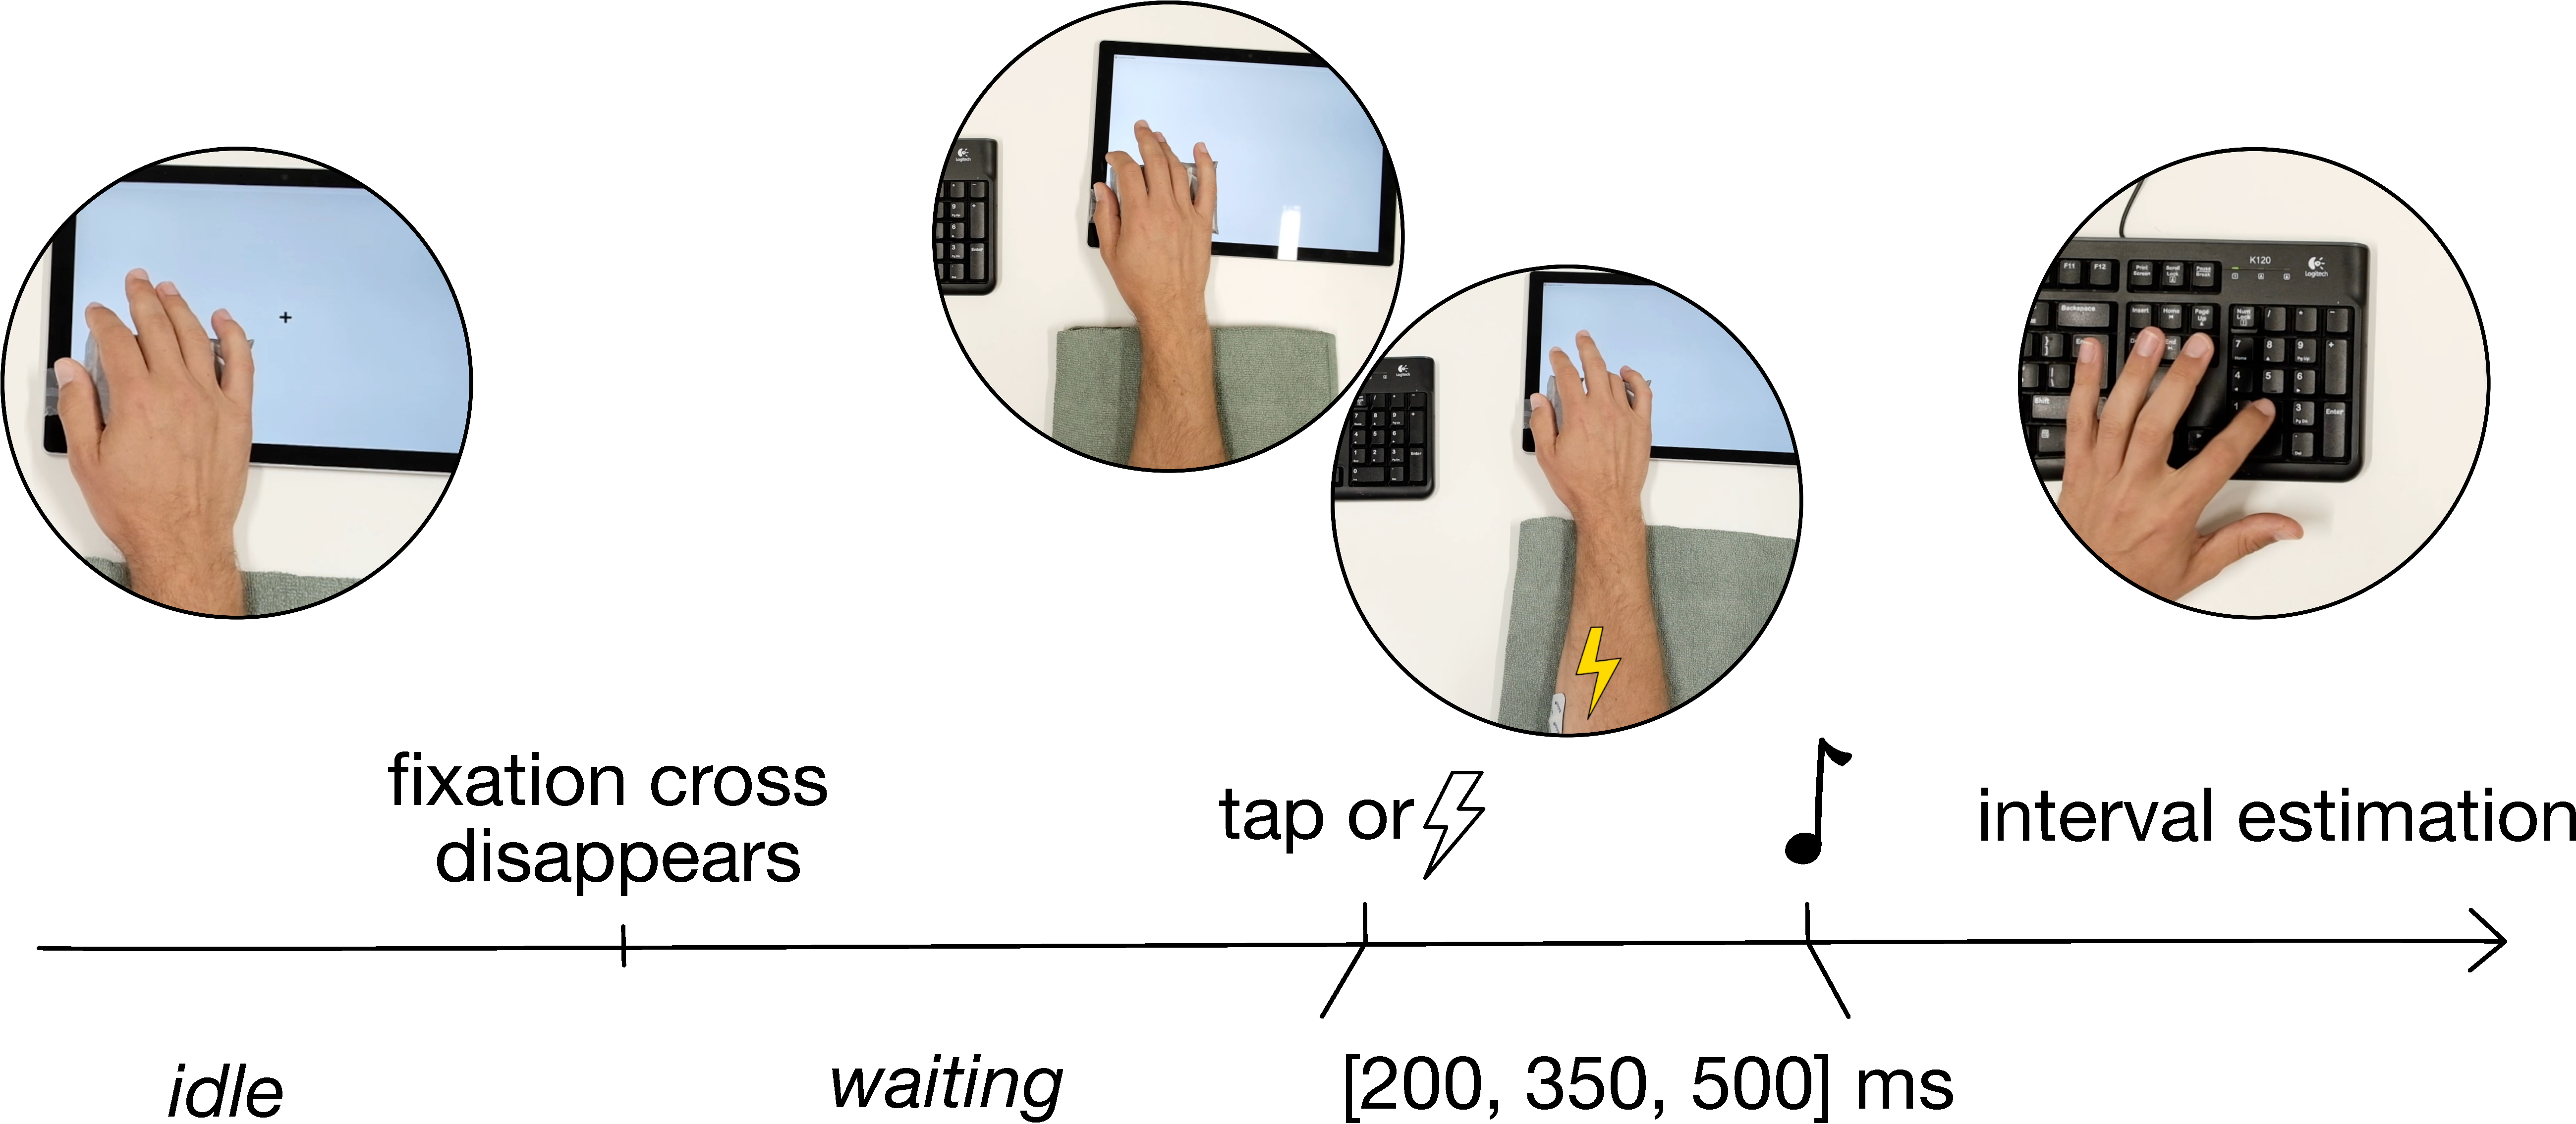
\includegraphics[width=\columnwidth]{figures/task_new.pdf}
    \caption{Interaction flow depicting one trial in our touchscreen tapping task.}
    \label{fig:progression}
\end{figure}

\indent\textbf{INTENTION.} The task was as follows: (1) a fixation cross appeared on a tablet screen and participants were instructed to rest and wait until it disappeared; (2) they were instructed to wait for a brief moment (2 to 3s), before (3) initiating their movement and tap the screen, see figure~\ref{fig:progression}. In line with the literature on the origin of the RP generating process, they were told ``to avoid pre-planning the movement, avoid any obvious rhythm across trials, and to press when they felt the spontaneous urge to move''~\cite{Schultze-Kraft2021-cu}. (4) After the screen was tapped, a tone was played at a pseudo-random delay of 200, 350, or 500ms. Participants were now asked to estimate the delay, typing in their answers on a number pad of an attached keyboard. After confirming their answer by hitting the return key, the next trial started.

During INTENTION, participants were equipped with \textcolor{red}{Electromyogram (EMG)}\textcolor{green}{EMG} sensors instead of EMS electrodes. \textcolor{red}{The EEG data from INTENTION was used as training data for the BCI, see section~\ref{BCI} below}. Participants' reaction times in INTENTION were used to select stereotypical reaction times for the EXTERNAL condition. At the end of INTENTION, EMG electrodes were exchanged for EMS electrodes at the identical location on the forearm.

% \textcolor{green}{The EMG data was used to detect muscle activity onsets, i.e. movement onsets. The detected onsets were then used to label the data of the \textit{pre-movement} class, see section~\ref{BCI} below for more details.}

\indent\textbf{EXTERNAL.} The task structure was identical to INTENTION, however, participants were now instructed to hold and wait for the muscle stimulation to move their finger thereby eliciting the screen tap. The timing for the EMS trigger was taken by randomly choosing a time between the 5th and 95th percentile of their actual individual reaction time in the INTENTION condition. 

\indent\textbf{AUGMENTED.} The task and instruction were identical to INTENTION with one additional instruction: ``you will now work \textit{with} the system''. During AUGMENTED, the muscle stimulation hardware was controlled by the BCI. The classifier was set to active after the fixation cross disappeared and until a screen tap was registered. Hence, the muscle was not stimulated at other times during a trial, so as not to interfere with participants typing in their time estimation response.

The order of the conditions was not pseudo-randomized since training data obtained in INTENTION was required for both EXTERNAL and AUGMENTED. Furthermore, AUGMENTED was always the last condition, thereby allowing for a prolonged interview~\textcolor{green}{immediately after the experience with the prototype.}

% alternative headings:
% Brain-Computer Interface to Detect EEG Readiness Potentials }
% Classifiying EEG Signals of the Intent to Interact
\subsection{Brain-Computer Interface}\label{BCI}
The data obtained in INTENTION was used to train the BCI. We utilized the [anonymized] and the EEGLAB~\cite{Delorme2004-sn} toolbox inside the MATLAB (The MathWorks Inc. Natick, MA, USA) environment for preprocessing both EEG and EMG data. First, to generate behavioral labels at a high temporal resolution for the EEG-based classifier, we leveraged EMG data from the flexor digitorum profundus. EMG amplitudes were band-pass filtered from 20 to 100 Hz and subsequently squared. Next, to label the time of movement onset, the EMG data was averaged across trials for the second preceding the screen tap. From this averaged data, the first sample where the EMG amplitude exceeded the 95th percentile was selected as the time of movement onset.
% TODO remove anonymization bemobil pipeline

% TODO/Ignore Next, noisy data segments were determined. 
% A segment was rejected as an outlier using Matlab's \textit{isoutlier} function using default parameters. % from isoutlier documentation (mean segment amplitude exceeding 3 scaled median absolute deviation)

Two event classes were then defined as follows: \textit{pre-movement} from -1000 to 0 ms preceding the (EMG detected) movement onsets and \textit{idle}, a one-second data segment between trials where participants were looking at a fixation cross.

\subsubsection{Preprocessing EEG and Selecting discriminative channels}\label{eeg_methods}
The EEG data was band pass filtered from 0.1 to 15 Hz. In the first step to prepare the EEG data for \textcolor{red}{classification}~\textcolor{green}{classifier training}, noisy data segments were rejected. To this end, the EEGLAB function `autorej' was used, keeping default parameters. A trial was excluded if \textit{either} data from the \textit{idle} or \textit{pre-movement} class was rejected.

Then, to decrease the dimensionality of the EEG data, we selected discriminative channels following an approach outlined by~\citep{Schultze-Kraft2021-cu}. First, for both \textit{pre-movement} and \textit{idle} the mean signal in the last 100 ms of each segment was subtracted from the mean signal in the first 100 ms of the segment. The resulting value thus indicated how much the signal had changed in the course of the 1 s segments. In line with the literature, there should be a change over time in the \textit{pre-movement} segment but not in the \textit{idle} segment. Then, all channels were sorted (1) in descending order by the signal difference in the \textit{pre-movement} segments and (2) in ascending order by the signal difference in the \textit{idle} segments. With respect to the ability of the system to discriminate between movement intention and the absence of movement intention, an ideal channel should show a strong change in signal over the course of a \textit{pre-movement} segment but no difference during an \textit{idle} segment. The ranks of the two criteria were joined by summation and the resulting order was saved for later use in training and real-time application of the classifier. Lastly, channels C3, C4, and Cz were moved to the top of the order for every participant as these are most frequently reported in studies on the RP.

\subsubsection{Training of EEG classifier}
To classify EEG data, a linear discriminant analysis (LDA) with shrinkage regularization (automatic shrinkage using the Ledoit-Wolf lemma~\cite{Ledoit2004-bi}) was trained for each participant individually. As single-trial features, the (linear) slope coefficient was obtained for both \textit{idle} and \textit{pre-movement} segments by fitting a linear regression. The classifier was then trained using the slope coefficient of the selection of the most discriminative channels as features, generating a feature vector in the dimension of channels that were kept for classification. We purposefully constrained the dimensionality of the feature vector to avoid over-fitting~\textcolor{green}{and decrease the computational load.}

Using scikit-learn~\cite{Pedregosa2012-sj}, the LDA \textcolor{red}{with automatic shrinkage} was cross-validated (using 5-folds) for a grid search from 6 to 20 channels with a step size of adding 2 channels. Following this grid search, the cross-validation with the highest accuracy determined the number of channels that were kept for training the model for real-time application. Ultimately, to determine the threshold at which, during the real-time application, the classifier would trigger the EMS, we computed the Receiver-operator characteristic (ROC) and from this selected the threshold at 15 \% false positive rate.

\subsubsection{Real-time application and EMS control}
During real-time application, the EEG data was buffered for the last second for the selected \textcolor{green}{discriminative channels}. The data was band-pass filtered analogously to the training data from 0.1 to 15 Hz. Next, the slope was computed. \textcolor{red}{for the discriminative channels selected in the classifier cross-validation grid search.} This procedure ran at an update rate of 10 Hz, hence every 100 ms a new prediction was obtained from the classifier. To smooth the prediction output to reduce false predictions due to unlikely peaks, the predicted probability for the \textit{pre-movement} class was smoothed by averaging the \textcolor{red}{last two} \textcolor{green}{current and the preceding prediction with a weighting (weight of .3 for the preceding, and .5 for the current prediction). The weights were obtained through trial-and-error during piloting}. Then, with a 10 Hz update rate, this smoothed probability, as well as the predicted class for the current frame were gating the EMS switch: when the probability exceeded the threshold and the currently predicted class was \textit{pre-movement}, the switch was opened for 0.5 s.

% To trigger the EMS, an Arduino was used to flip a switch whenever triggering the attached EMS. We constrained the times when the switch could be flipped to specific moments in the experiment where participants were getting ready to perform an action, thereby limiting the impact of distracting EMS pulses at resting phases during the experimental trials. %This guaranteed that participants experienced EMS only during movement preparation

\subsection{Measures of Agency Experience: Intentional Binding, Question \& Interview}
To assess if SoA was preserved, an intentional binding measure, a standardized question, and an interview following the AUGMENTED block were investigated. After each condition we prompted participants to rate their experienced agency on a 7-point Likert scale with the statement ``It felt like I was in control of the movements during the task.'', the item was copied from~\cite{Bergstrom2022-fb}. Following AUGMENTED we interviewed users about their experience working with the system. After prompting users to recall their experience and summarize what their task had been, we set the focus to the tapping movement and asked them to ignore the time estimation task in the questions that followed. We entered the open part of the interview by asking: ``What did the system do?'' followed up by ``What was the difference between the three conditions''. After some time, and depending on their answers, we reset the focus to the AUGMENTED condition and asked ``How often was the system active?'' followed by ``What do you think caused the actions of the system?''. This was then followed up by an `open' interview in which we frequently asked `how' and `why' questions to inquire about the user's experience.

% add back in after anonymization: All interviews were manually transcribed and then automatically translated using }
We analyzed the interviews \textcolor{red}{that always followed the AUGMENTED condition} by loosely following~\citet{Mayring2015-pp}. All interviews were manually transcribed and translated to English using DeepL\footnote{https://www.deepl.com/translator} (DeepL SE, Cologne, Germany). Before screening the texts, two experts clustered the responses into 3 clusters: First, ``Functionality'' referred to what participants attributed the source of the stimulation. Next, we clustered responses according to ``Guessed percentage'' of correct interaction, i.e., participants' estimate of how well the system was aligned with their intention. For the cluster ``Correct Interaction'', we specifically queried participants to recall the moments where the stimulation felt in line with their intention to move, then we clustered their responses into sentiments with positive and negative valence. 

\subsection{Statistical Analyses}
To confirm and demonstrate the discriminative power of the EEG features, we plotted the amplitude time course of electrode Cz between \textit{pre-move} and \textit{idle} epochs. \textcolor{green}{Electrode Cz was chosen for exemplary presentation, as it is frequently reported in studies on the RP, since it captures neural activity originating from the sensorimotor cortex.} Next, the slope coefficients were extracted and a paired t-test was conducted. Ultimately, to assess the classifier performance, we calculated the F1 score, i.e. the harmonic mean of precision and recall, and plotted the ROC\textcolor{green}{, see figure~\ref{fig:EEG_results} a to c.}

\subsubsection{Hypotheses Testing}
Prior to any statistical analyses of the intentional binding measure, outlier trials were rejected. We applied `extreme outlier removal' using Tukey's method~\cite{Tukey1949-sl}. Three time intervals were considered relevant to describe `regular' behavior across trials which would manifest by: (1) Tapping the screen in a reasonable interval after the fixation cross disappeared. An excessively short or long delay indicated that participants either tapped the screen prematurely by accident or they were checking in with the experimenter, respectively. (2) Providing a `reasonable' estimation in the intentional binding task. (3) The EMS stimulation leading to an \textit{immediate} screen tap. A long delay between the EMS trigger and the subsequent screen tap indicated that the stimulation was not strong enough in this trial to lead to muscle actuation resulting in a screen tap. Taken together, applying Tukey's method \textcolor{green}{to each of these time windows and fusing the rejected trials} \textcolor{red}{criteria} led to the exclusion of 102 trials across all participants (M = 34.00, SD = 16.46) and a final data set of 1698 trials.

In line with the literature on intentional binding, we hypothesized that the time intervals should be underestimated for the INTENTION and the AUGMENTED conditions. This should not be the case for the EXTERNAL condition where users had no intention to move. Hence, when binding occurs, the intervals should be underestimated, hinting at a higher SoA. To test this, we fitted a linear mixed effects model with \textit{condition} (INTENTION, EXTERNAL, AUGMENTED) as a fixed effect and as a random effect, we considered the intercepts for participants \textcolor{green}{($time interval ~ condition + 1|participantID$)}. We obtained p-values of the coefficients by calculating likelihood-ratio tests. All parameters were estimated by maximum likelihood estimation~\cite{Pinheiro2006-bk}. Post hoc, \textcolor{green}{we computed pairwise contrasts with the Tukey HSD (Honest Significant Differences), accounting for multiple companions with alpha correction~\cite{Lenth2020-xk}.}
% ~\cite{winterLinearModelsLinear2013}

Next, we hypothesized that subjective ratings of control over the tap movement are comparable between INTENTION and AUGMENTED and lower in the EXTERNAL condition. Again, we fitted a linear mixed effects model with \textit{condition} as a fixed effect and participant ID as a random effect. Coefficients were assessed in the same way as for the intentional binding parameter above.

In short, we tested two main hypotheses with regard to the agency experience in our three experimental conditions: (1) participants underestimate the tone delay when acting intentionally. Adding EMS in line with participants' intention to move does not affect this underestimation. (2) The subjective feeling of control is comparable between INTENTION and AUGMENTED conditions. EXTERNAL should decrease the feeling of control significantly. Additionally, we report the clustered interviews anecdotally.


%%% Resources
\begin{comment}

% An additional cluster ``takeaways'' was used to cluster other, miscellaneous,  interesting comments.

% "how did it feel like?". If user's made reference themselves to the EMS device we followed up by inquiring: "why do you think it (the EMS trigger) happened?", "What do you think triggered it?". The goal was to learn about the source attribution user's made about the EMS trigger. Since we leveraged the RP, we hypothesized that user's would attribute, at least in part, the EMS trigger to themselves, i.e. their movement intention. Next, we pressed deeper into learning about the cooperative nature between user and system. We asked "Do you believe you did it alone?" and when they made reference to a specific situation where the EMS was triggered we followed up with "What did it feel like, did you had the feeling the system controlled you or did you cooperate?" and "What would have to be there for it to feel like a cooperation?". We closed the interview with two additional exploratory questions: "Did the system influence your performance? If yes, how and why?" as well as asking them about any application scenarios they have in mind. 

% \indent\textbf{(1) Intentional Binding.}
% At the end of each trial participants were tasked to estimate the delay between the screen tap and a subsequent tone. The real delay was pseudo-randomized out of [200, 350 and 500] ms. With 75 trials per condition, each real delay occurred 25 times. 

% \indent\textbf{(2) Questionnaire.}

% \subsection{Brain-Computer Interface}
% The presented classification scheme required individual training data per participant, as transfer learning remains challenging with EEG~\cite{Wan2021-zz}. Therefore, we initially obtained training data on a variant of our task that did not include any muscle stimulation. In our task, participants were instructed, following an initial waiting period, to tap a touchscreen with their ring finger at their own volition, see figure ~\ref{fig:teaser}. 
% \subsubsection{Labelling movement classes using EMG}3

% Subsequently the data were labelled into two classes: an \textit{idle} class representing resting background activity and a \textit{pre-movement} class, representing the intent to (inter-)act.

% In summary, the experiment consisted of five phases: (1) a setup phase; (2) the BASELINE condition to obtain training data and labels; (3) the NO INTENTION condition: being passively moved by the EMS system; (4) the INTENTION EMS condition where the BCI was triggering the EMS system that in turn made participants tap the screen; and (5) an open interview to inquire about their experienced agency following the INTENTION EMS condition.

% \subsubsection{Experiment Design and Procedure}
% The first condition was used to obtain training data for the single-trial classification system. Here participants were wearing the EMG sensors instead of the EMS actuators and were instructed to tap the screen at their own volition (BASELINE, see instructions above). In the second condition, participants were instructed to hold and wait for the EMS system to move their finger thereby eliciting the screen tap (NO INTENTION). The timing for the EMS trigger was taken by randomly choosing a time between the 5th and 95th percentile of their actual reaction time in the BASELINE condition. In the third condition, the EMS trigger was controlled through the readiness potential classifier (INTENTION EMS). Participants were given the instruction: ``you will now work \textit{with} the system'' along the same instruction as in the BASELINE condition. The classifier was set to active after the fixation cross disappeared and until a screen tap was registered. Hence, the EMS was not triggered at other times during a trial, so as not to interfere with participants typing in their time estimation response.

% To not break the user's immersion by disturbing the flow of the interaction we decided against asking qualitative questions at the end of each and every trial.

% old:
% \subsubsection{Reproducing Results and Data Availability}
% Data, experimental protocol, analyses code including scripts for a reproduction of the presented results are hosted at open science foundation (OSF)\footnote{[anonymized]}. BIDS formatted data is hosted on openneuro~\cite{}.


% , and the interval between EMS stimulation and tap as fixed effects

% Hypothese:
% In line with the literature on intentional binding, we hypothesized this duration to remain stable in the case that agency was preserved during the test phase with EMS. A deviation of the tone duration from the training phase was hypothesized to reflect a disruption in experienced agency.

% operationalising temporal binding = underestimation (here or somewhere else) 

% \indent\textbf{(1) Hand Tracking.} We used an HTC Vive Tracker, attached to the participant's wrist, to track their right hand at 90Hz. Therefore, we ran a simple Unity3D scene and streamed the data via the labstreaminglatyer (LSL)\footnote{https://github.com/sccn/labstreaminglayer}

% At the end of each trial participants were tasked to compare the duration of their arm movement to a tone and indicate whether the tone was longer or shorter. We set the initial duration at 500 ms for each participant. When participants indicated the tone to be longer or shorter by pressing either the up or down key we added, or respectively subtracted, 100 ms from the tone duration. This new duration was then used for the next trial and so on. With 60 trials in the training phase, we hypothesized participants would oscillate 50-50 around a target duration after about 2/3 of the training trials. The final duration after all training trials was then used again as the start duration during the test phase. In line with the literature on intentional binding, we hypothesized this duration to remain stable in the case that agency was preserved during the test phase with EMS. A deviation of the tone duration from the training phase was hypothesized to reflect a disruption in experienced agency.


% (1) participants waited for a new letter to appear on screen; (2) then, they were instructed to wait for a brief moment (~2s), before (3) reaching out and pressing the key. In line with the literature on the origin of the RP generating process they were told "to avoid preplanning the movement, avoid any obvious rhythm, and to press when they felt the spontaneous urge to move". (4) Two \todo{how many, but do keep this constant in order for them to focus on the duration of their action} seconds after they pressed the key, they were presented with a tone and asked to judge whether their movement, from the start of their reach to the button press, lasted longer or shorter than the tone. (5) When they perceived the tone to be longer, they had to press the up key or vice versa the down key for perceiving that the tone was shorter than their movement. Following an inter-trial-interval the next trial started.

% For each trial, a key was randomly selected from one of two groups of letters: (1) 'a', 's', 'd' or (2) 'j', 'k', 'l'. The selected group was then changed with every trial. This was done to keep the task engaging while maintaining a comparable reaching movement between trials.

% ERP with significance mask for Cz? Assessing significance of classifier

% IB Task: ttest of final ib time between with and without EMS -> # subjects input values
% did they increase the IB task in more than 50% of the trials after EMS?

% questionnaires: ttest against zero to report direction

% interviews: anecdotal summary and sentiment analyses with two groups splitting questionnaires at 0

% correlation with EEG classifier accuracy?

% evaluation of EEG classifier: can report false negatives, how often was it missing to predict a movement onset? hand was moving without EMS being triggered occurred how often? Not possible to evlaute false positives as no ground truth available

\end{comment}